% \section{01 section}
% \label{sec:01label}

%% Template
% \begin{frame} \frametitle{01 Title}
%     \framesubtitle{02 Maybe Subtitle}
%     \begin{block}{01 1 Maybe a Block}
%         Hi
%     \end{block}
%     \begin{block}{01 2 Maybe a Block}
%         Hi
%     \end{block}
% \end{frame}






\begin{frame} \frametitle{Motivation}
    \begin{itemize}
    % \item Not another semester project
    \item Make something needed
    \item Satlab -- Improve receiver for ground station
    \end{itemize}

\begin{figure}[htbp]
    \centering
    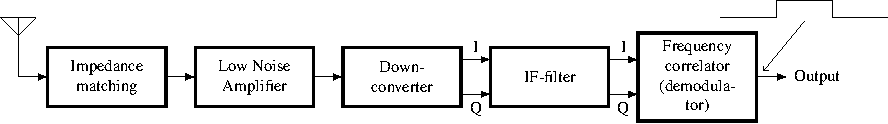
\includegraphics[width=0.9\textwidth]{img/adf7021}
    % \caption{Existing setup for the hardware based radio receiver based on the ADF7021}
    \label{fig:adf7021}
\end{figure}

\begin{itemize}
    \item Better reception
    \item More Flexible
    \item Soft-bit decision
\end{itemize}

% \begin{figure}[htbp]
%     \centering
%     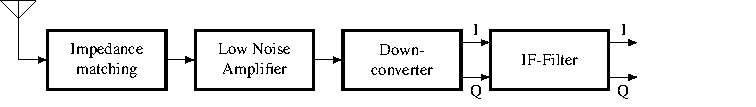
\includegraphics[width=0.9\textwidth]{img/front_end}
%     % \caption{Front end for this project}
%     \label{fig:front_end}
% \end{figure}
\end{frame}


\section{Modulation Scheme}
\begin{frame} \frametitle{Modulation Scheme -- FSK}
\begin{figure}[htbp]
    \centering
    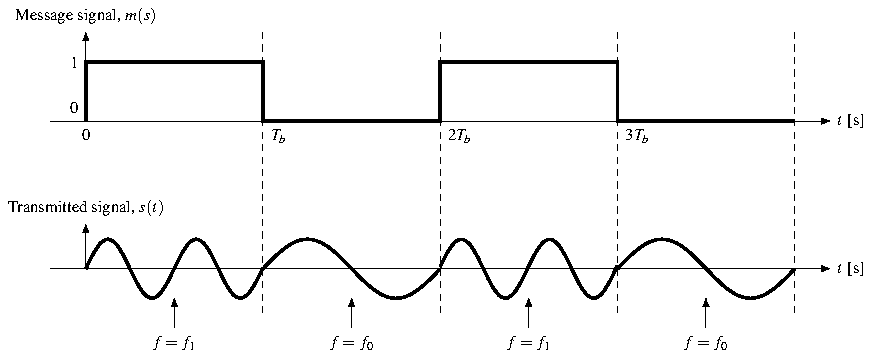
\includegraphics[width=0.9\textwidth]{img/gfsk_basics}
    % \caption{Example of FSK modulated signal. Binary message signal on top and modulated signal below. It is seen that the frequency is lower---$f_0$---at a 0-transmission than at a 1-transmission---$f_1$. Here the modulation index is $h=1$}
    \label{fig:gfsk_basics}
\end{figure}
\begin{itemize}
    \item FSK -- Frequency Shift Keying 
\end{itemize}

    \begin{equation}
    \label{eq:msk_mod_output1}
    s(t) = \sqrt{\frac{2E_b}{T_b}} \cos{[2\pi f_c t + \phi(t)]}
    \end{equation}
    \begin{equation}
    \phi(t) = \phi(0) \pm {h\pi t}/{T_b}
    \end{equation}

    \begin{equation}
    \Delta f = |f_1-f_0| = \frac{h}{T_b} = \frac{1}{ \frac{1}{9600} } = 9600 \text{ Hz}
    \end{equation}
\end{frame}

\begin{frame} \frametitle{Modulation Scheme -- GFSK}
\begin{figure}[htbp]
    \centering
    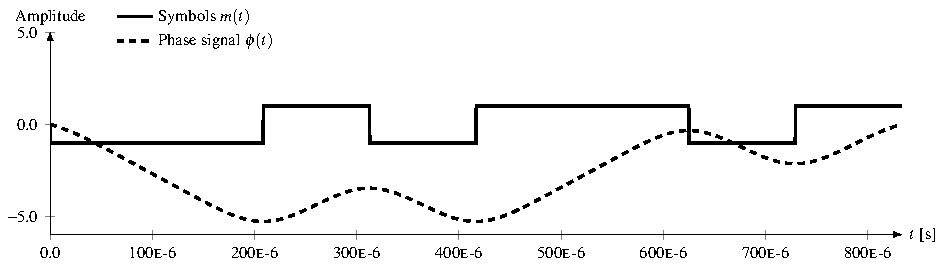
\includegraphics[width=0.9\textwidth]{img/gfsk_integration}
    % \caption{To calculate $\phi(t)$ when the input sequence is filtered, an integral and scaling may be used. Above is shown integration of an unfiltered NRZ sequence to show the correlation to Equation~\ref{eq:msk_mod_output1}. Above: NRZ signal $m_{\text{NRZ}}(t)$. Below: Integrated and scaled signal $\phi(t)$.}
    \label{fig:gfsk_integration}
\end{figure}
\begin{itemize}
    \item $ \phi(t) = \phi(0) + \frac{h\pi}{T_b}\int_{0}^{T_b} m_{\text{NRZ}}(t)  dt$
    \item Basis for demodulating by phase
\end{itemize}
\end{frame}

\section{Spacelink Format}
\begin{frame} \frametitle{Spacelink Format}
    \begin{figure}[htbp]
        \centering
        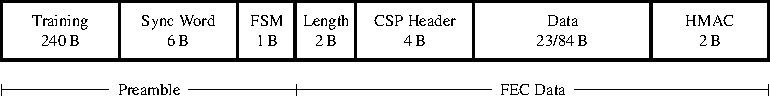
\includegraphics[width=0.9\textwidth]{img/spacelink_format}
        % \caption{CSP packet\cite{aausat3spacelink}.}
        % \caption{CSP packet.}
        \label{fig:spacelink_format}
    \end{figure}

\begin{itemize}
    \item Recording from AAUSAT III
\end{itemize}
    \begin{figure}[htbp]
        \centering
        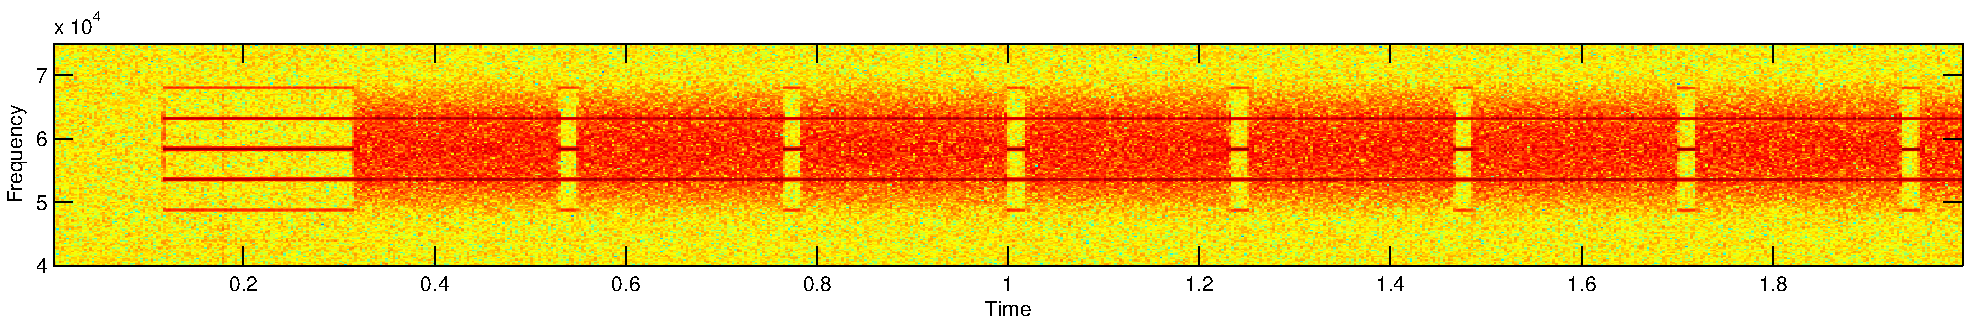
\includegraphics[width=1\textwidth]{img/packet_from_recording}
        % \caption{Recording of a burst from a pass of AAUSAT3, sampled with \SI{192}{k\hertz}..}
        \label{fig:packet_from_recording} 
    \end{figure}

\begin{itemize}
    \item Signal generator
    \item  $\text{Short package} = 8 \cdot \left( 24B+6B+1B+128B \right) = 1272 \text{ Symbols}$
\end{itemize}
    
\end{frame}


\section{Blackfin Architecture}
\begin{frame} \frametitle{Blackfin Architecture}
    \begin{figure}[htbp]
      \centering
      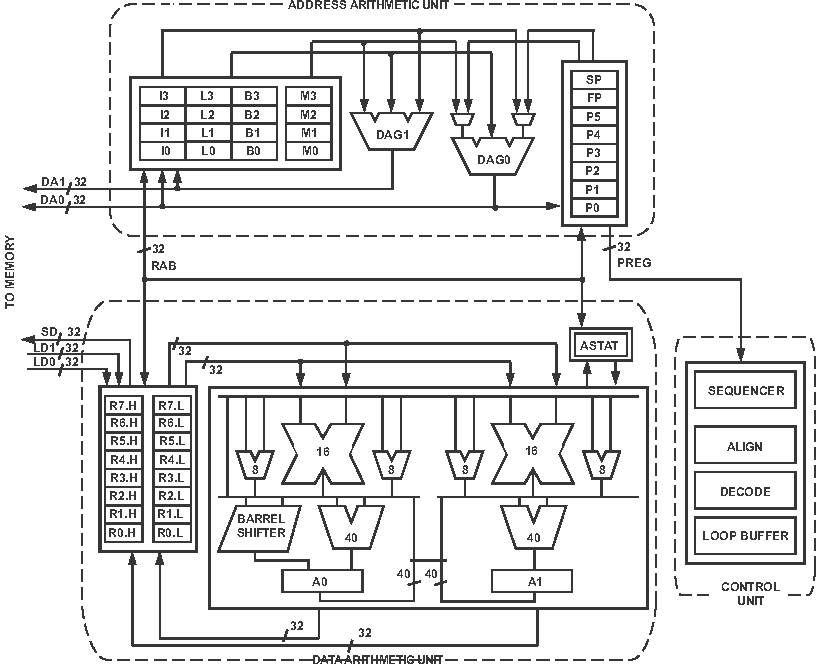
\includegraphics[width=0.9\textwidth]{img/bf537_internal}
      % \caption{The core of the Blackfin BF537.}
      % \caption{The core of the Blackfin BF537.\cite{bf637ShortReference}}
      \label{fig:bf537_internal}
    \end{figure}
\end{frame}


\section{Program Flow}
\begin{frame} \frametitle{Division Into Sub Modules -- Program Flow}
    \begin{figure}[htbp]
        \centering
        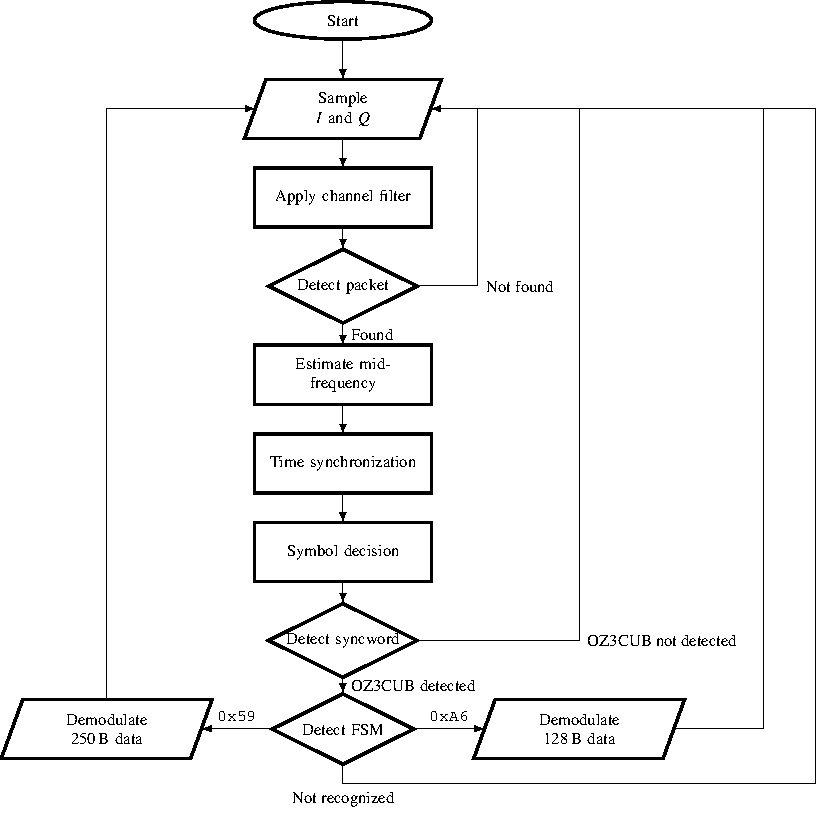
\includegraphics[height=0.8\textheight]{img/program_flow}
        \caption{Program flow after implementation.}
        \label{fig:programflow1}
    \end{figure}
\end{frame}

% \section{Interfaces}
% \begin{frame} \frametitle{Interfaces}
%     \begin{figure}[htbp]
%         \centering
%         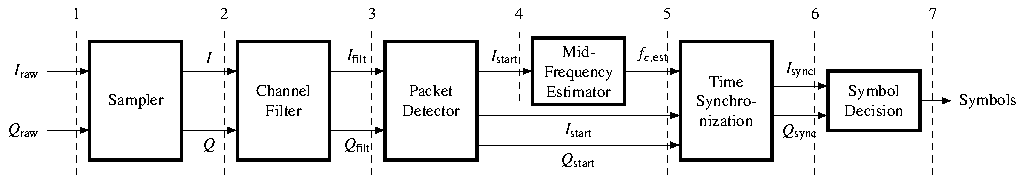
\includegraphics[width=1\textwidth]{img/interfaces}
%         % \input img/interfaces
%         \caption{Interfaces between modules}
%         \label{fig:Interfaces}
%     \end{figure}
% \end{frame}



